\documentclass{beamer}

\usetheme{Copenhagen}
%% \usenavigationsymbolstemplate{}
\setbeamertemplate{navigation symbols}{}
%% \usecolortheme[rgb={0.4,0.5,0.4}]{structure}
\usepackage{color}
\usepackage{listings}
% \usepackage[T1]{fontenc}
% \usepackage{libertine}
\usepackage[spanish]{babel}
\usepackage[utf8]{inputenc}
\usepackage{graphicx}
\usepackage{verbatim}
\usepackage{hyperref}
%\usepackage{wrapfig}
\usepackage{siunitx}
\usepackage[version=3]{mhchem}
\usepackage{multicol}

\graphicspath{ 
	{../../FEM_termico/celula/scripts/itvs/}
	{../../FEM_termico/celula/scripts/curvas/}
	{../../FEM_termico/celula/scripts/poros/}
	{../../FEM_termico/AutoMesh2D/grande/}
}

\title{Electroporación celular}
      
\author{Mauricio Alfonso}
\institute{DC - FCEyN - UBA}
%\date[11.2013]{SegInf, 2c - 2013}

%TODO poner subsections en cada frame!
%TODO sacar lo que sobre (explicaciones de cada constante, etc)
%TODO badboxes

\begin{document}
	\newcommand{\h}{\ce{H^+}}
	\newcommand{\oh}{\ce{OH^-}}
	\newcommand{\na}{\ce{Na^+}}
	\newcommand{\cl}{\ce{Cl^-}}
	\newcommand{\kvm}{$\si{\kilo\volt\per\metre}$}
	\newcommand{\usec}{$\si{\micro\second}$}

	\begin{frame}
		\titlepage
	\end{frame}

	\section{Introducción}
		\frame{
			\begin{itemize}
				\item Una célula esférica de entre 10 y 50 \si{\micro\metre} de radio
				\item Dos electrodos que generan un pulso de 20 \si{\milli\second} de entre 40 y 200 \kvm
				\item Se estudia la generación de poros en la membrana celular y el ingreso de \h, \oh, \na{} y \cl{} a la célula.
				
			\end{itemize}
		}
	
	\section{Mallado}
		\frame{	
			\begin{multicols}{2}
				\begin{itemize}
					\item Coordenadas cilíndricas (2D)
					\item Elementos cuadrilaterales
					\item Programa AutoMesh2D para generar mallas
					\item 2 mallas diferentes: una de 1930 elementos y otra de 7439 elementos
				\end{itemize}
			\columnbreak
				\begin{center}
					%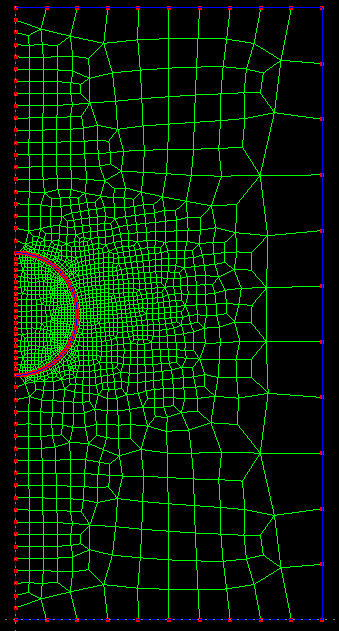
\includegraphics[keepaspectratio,width=.6\textwidth]{grande} \\
					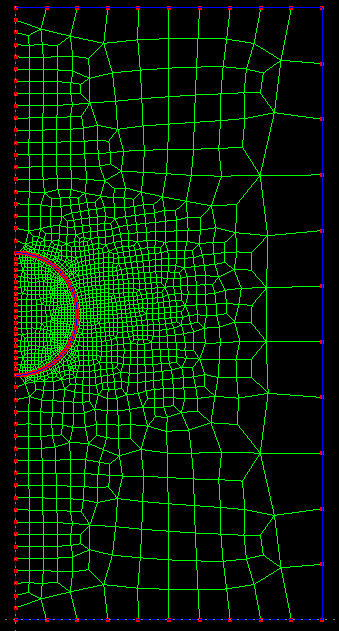
\includegraphics[keepaspectratio, height = 0.95\textheight]{grande} \\
					%Ejemplo de malla
				\end{center}
			\end{multicols}
		}
		
%		\frame{
%			\begin{center}
%				%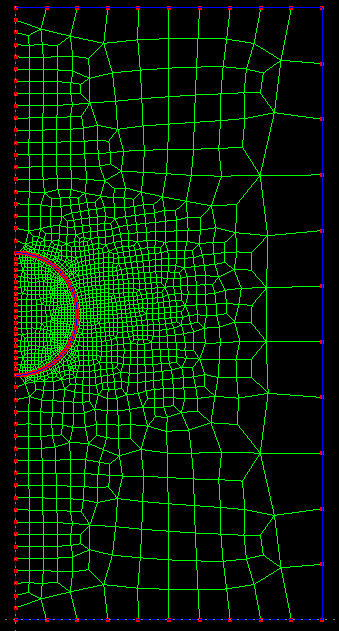
\includegraphics[keepaspectratio,width=.6\textwidth]{grande} \\
%				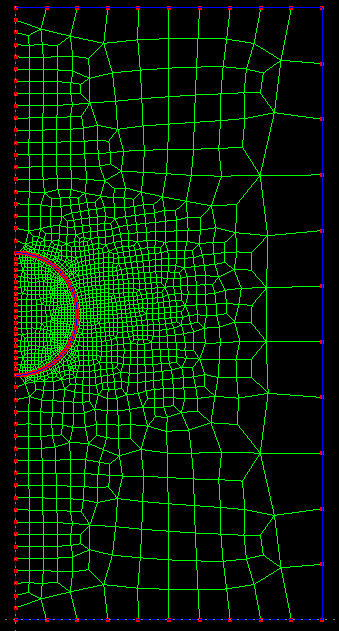
\includegraphics[keepaspectratio, height = \textheight]{grande} \\
%				%Ejemplo de malla
%			\end{center}
%		}
	
		\frame{
			\begin{center}
				%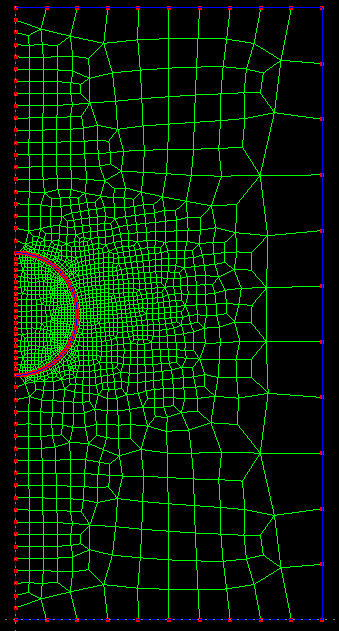
\includegraphics[keepaspectratio,width=.6\textwidth]{grande} \\
				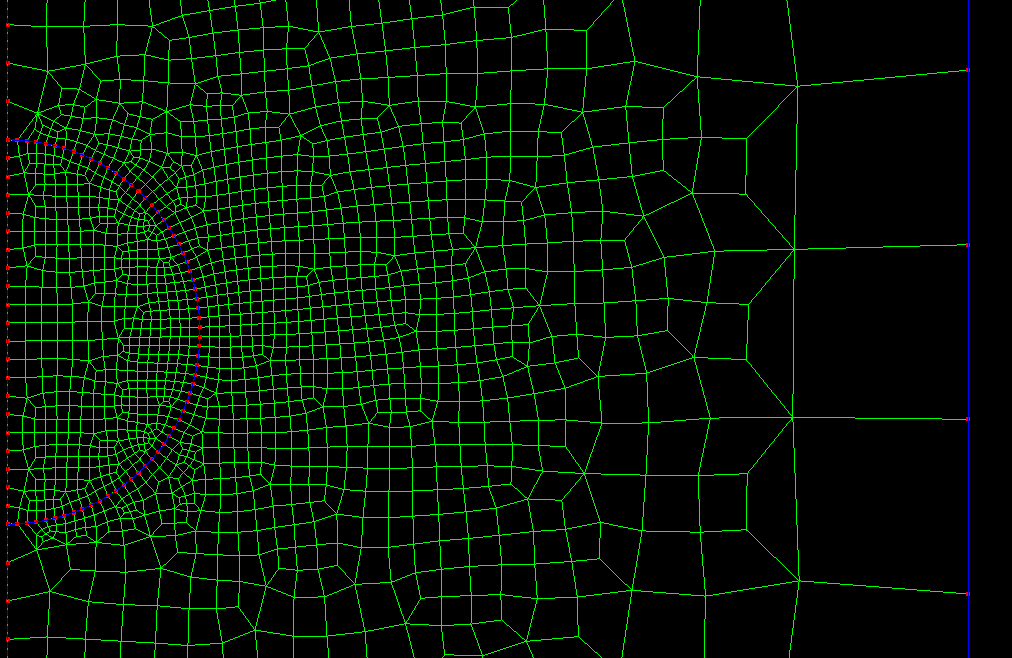
\includegraphics[keepaspectratio, height = 0.95\textheight]{grande2} \\
				%Ejemplo de malla
			\end{center}
		}

	\section{Potencial Eléctrico}
		\frame{
			Potencial eléctrico:
			\begin{center}
				$\nabla \sigma_{elem} \cdot (\nabla \phi) = 0$
			\end{center}
			Condiciones de borde de Dirichlet en los electrodos y Neumann en los otros bordes.\\
			
			El potencial transmembrana (ITV) debería aproximarse a:
			\begin{center}
				$V^{\theta} = 1.5 E cos (\theta)$
			\end{center}
		}
		
		\frame{
			Capacitancia de la membrana:
			FALTA ESTO!!!!
		}
		
	%	ACÁ PODRÍA IR UN DELAUNAY DE POTENCIAL O CAMPO!!!
	
	\section{Generación de poros}
		\frame{
			Generación de poros (densidad):
			\begin{center}
				$\frac{\partial N}{\partial t} = \alpha_c e^{(V_m/V_{ep})^2} \left( 1 - \frac{N}{N_0 e^{q \left(V_m/V_{ep} \right) ^2}} \right)$
			\end{center}
			$N$ es la densidad de poros en un determinado tiempo y posición de la membrana celular, $\alpha_c$ es el coeficiente de creación de poros, $V_m$ es el potencial transmembrana, $V_{ep}$ es el voltaje característico de electroporación, $N_0$ es la densidad de poros en equilibrio (cuando $V_m = 0$) y $q$ es una constante igual a $(r_m / r*)^2$, donde $r_m$ es el radio de mínima energía para $V_m = 0$ y $r*$ es el radio mínimo de los poros.\\
			
			La densidad depende del ángulo (no es constante en toda la superficie).
		}
	
		\frame{
			Radio de los poros:
			\begin{center}
				$\frac{\partial r}{\partial t} = \frac{D}{kT} \left( \frac{V_m^2 F_{max}}{1+r_h / (r+r_a)} + \frac{4 \beta}{r} \left(\frac{r_*}{r}\right)^4 - 2 \pi \gamma + 2 \pi \sigma_{\textrm{\tiny eff}} r\right) ,$
			\end{center}
			
			\begin{center}
				$ \textrm{con } \sigma_{\textrm{\tiny eff}} = 2 \sigma^\prime - \frac{2 \sigma^\prime - \sigma_0}{(1 - A_p / A)^2}	$
			\end{center}		
			
			Se aplica a cada poro por separado. Modela como crece el radio de los poros, y como se vuelven a sellar si baja el ITV.
			
			El primer término corresponde a la fuerza eléctrica inducida por el potencial transmembrana, el segundo a la repulsión estérica, el tercero a la tensión de línea que actúa en el perímetro del poro y el cuarto a la tensión superficial de la célula.
		}
	
		\frame{
			Donde $r$ es el radio de un poro, $D$ es el coeficiente de difusión para los poros, $k$ es la constante de Boltzmann, $T$ la temperatura absoluta, $V_m$ el potencial transmembrana, $F_{max}$ la máxima fuerza eléctrica para $V_m$ de 1V, $r_h$ y $r_a$ son constantes usadas para la velocidad de advección, $\beta$ es la energía de repulsión estérica, $\gamma$ es la energía del perímetro de los poros, y $\sigma_{\textrm{\tiny eff}}$ es la tensión efectiva de la membrana, $\sigma^\prime$ es la tensión de la interfase hidrocarburo-agua, $\sigma_0$ es la tensión de la bicapa sin poros, $A_p$ es la suma de las áreas de todos los poros en la célula, y $A$ es el área de la célula. 
		}	
	
	\section{Transporte}
		\frame{
			Transporte de especies: Nernst-Planck
			\begin{center}
				$\frac{\partial C_i}{\partial t} = \nabla \cdot \left( D_i \nabla C_i + D_i z_i \frac{F}{R T} C_i \nabla \phi \right)$
			\end{center}
			$C_i$ es la concentración de la especie $i$, $D_i$ el coeficiente de difusión de la especie $i$, $z_i$ la valencia de la especie $i$, $F$ la constante de Faraday, $R$ la constante de los gases y $T$ la temperatura.					
		}

	\section{Implementación}
		\frame{
			\begin{block}{Implementación}
				\begin{itemize}
					\item Métodos de elementos finitos para potencial eléctrico (ecuación de Poisson) y transporte de especies
					\item Diferencias finitas para generación y evolución de poros
					\item Implementado en \texttt{C++}
					\item Librería Eigen para resolver sistemas de ecuaciones
					\item Descomposiciones Cholesky (para Poisson) y Bi-gradientes conjugados estabilizados (para transporte)
					\item OpenMP para acelerar llenado de matrices (Poisson) y resolución en transporte
				\end{itemize}
			\end{block}
		}

	\section{Resultados}
		\subsection{ITV vs tiempo (inicio)} \frame{
			\begin{multicols}{2}
				\begin{figure}
					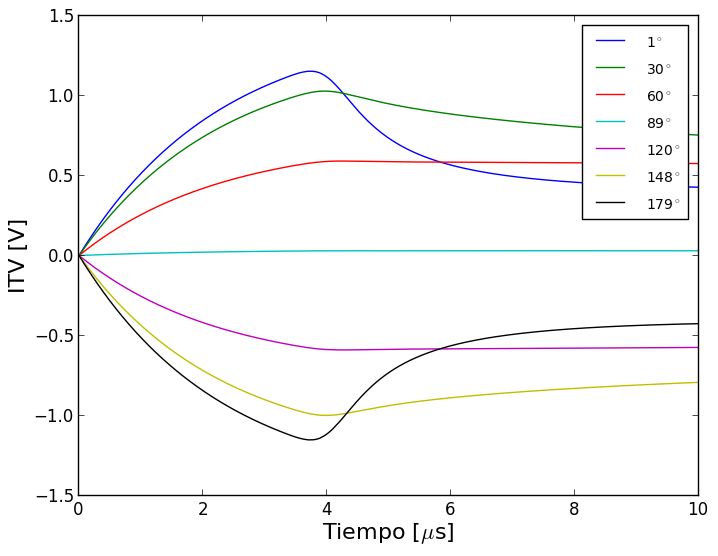
\includegraphics[keepaspectratio, width=0.5\textwidth]
						{itv-time-lin-25-64-40KVm}
					\caption{Para $\alpha$ = 25\si{\micro\metre} y 40\kvm}				
				\end{figure}
			\columnbreak
				\begin{figure}
					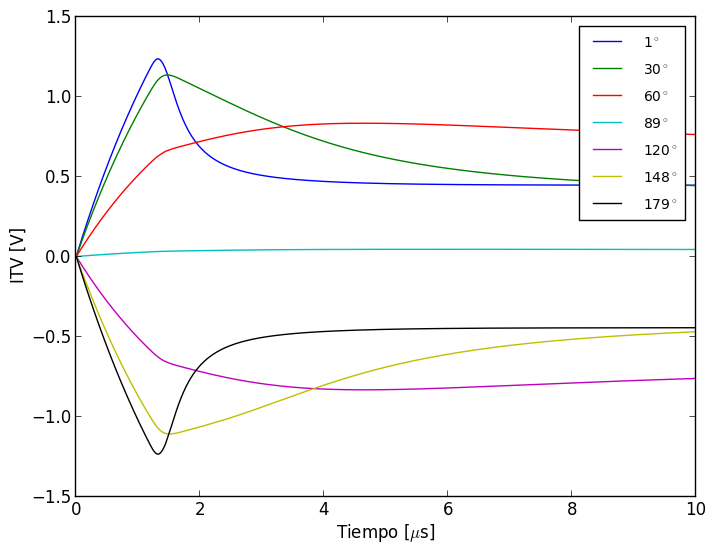
\includegraphics[keepaspectratio, width=0.5\textwidth]
						{itv-time-lin-25-64-80KVm}
					\caption{Para $\alpha$ = 25\si{\micro\metre} y 80\kvm}
				\end{figure}
			\end{multicols}
		}
				
		\subsection{ITV vs ángulo (pulso)} \frame{ 
			\begin{center}
				\begin{figure}
					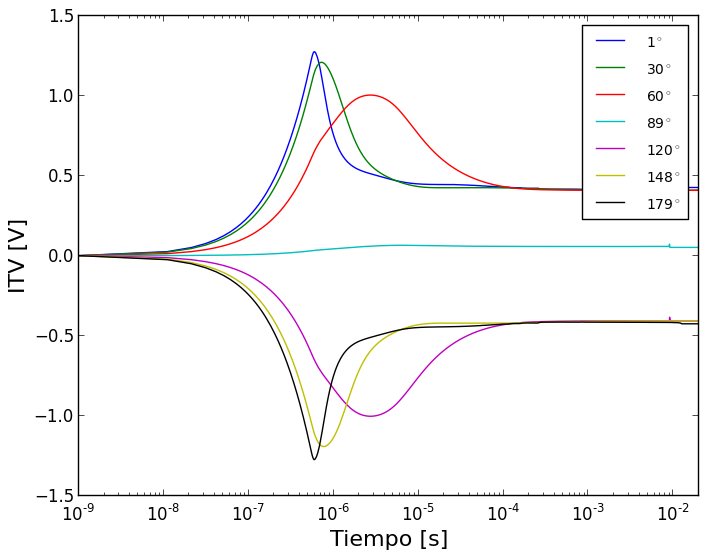
\includegraphics[keepaspectratio, height=0.85\textheight]
						{itv-time-log-25-64-160KVm}					
					\caption{Pulso entero para para $\alpha$ = 25\si{\micro\metre} y 160\kvm}
				\end{figure}
			\end{center}
		}
		
		\subsection{ITV vs ángulo} \frame{
			\begin{center}
				\begin{figure}
					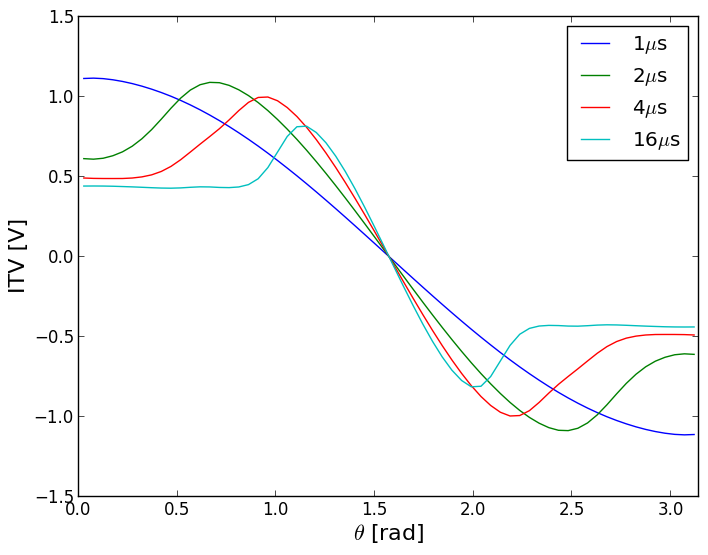
\includegraphics[keepaspectratio, height=0.85\textheight]
						{itv-tita-50-64-80KVm}					
					\caption{$\alpha$ = 50\si{\micro\metre} y 80\kvm}
				\end{figure}
			\end{center}
		}
		
		\subsection{Distribución de poros grandes según radio} \frame{
			\begin{multicols}{2}
				\begin{figure}
					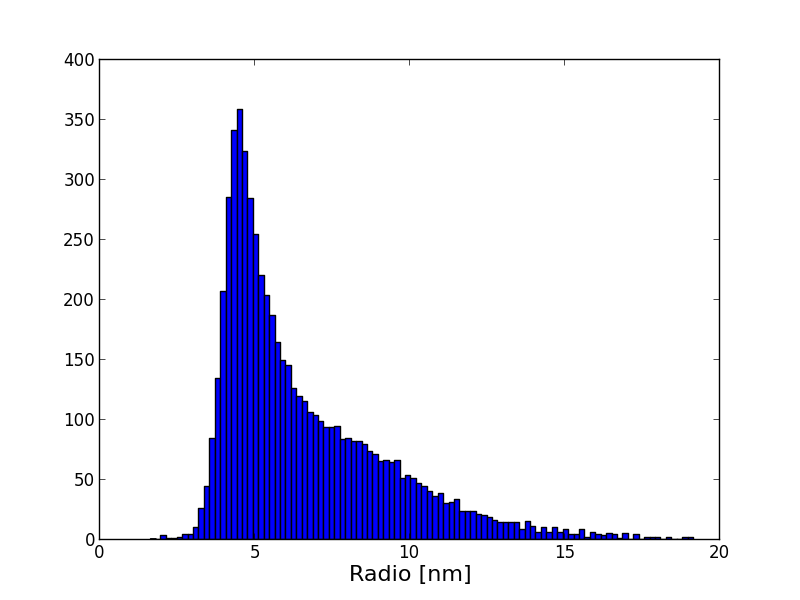
\includegraphics[keepaspectratio, width=0.56\textwidth]
						{hist-radios-5e-6-50-64-160KVm}
					\caption{Para $\alpha$ = 50\si{\micro\metre}, 40\kvm y t = 5 \usec}
				\end{figure}
			\columnbreak
				\begin{figure}
					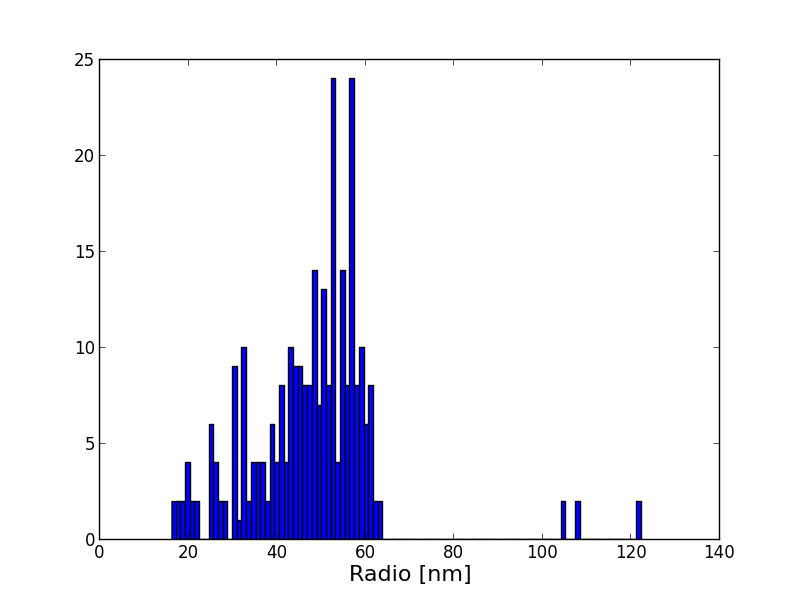
\includegraphics[keepaspectratio, width=0.56\textwidth]
						{hist-radios-5e-3-50-64-160KVm}
					\caption{Para $\alpha$ = 50\si{\micro\metre} y 160\kvm  y t = 5 \si{\milli\second}}
				\end{figure}
			\end{multicols}
		}
					
		
		
	\section{Trabajo Pendiente}

\end{document}
